%%%%%%%%%%%%%%%%%%%%%%% preamble %%%%%%%%%%%%%%%%%%%%%%%%%%%
\documentclass[10pt,letterpaper]{article}
\usepackage{opex3}
\usepackage{amssymb}
\usepackage{hyperref}
\hypersetup{colorlinks=true,
		      urlcolor=blue}
\usepackage{amsmath}      
\usepackage{listings}
\lstdefinestyle{mybashstyle}{
  language=Python,
  numbers=none,
  stepnumber=1,
  numbersep=10pt,
  tabsize=4,
  showspaces=false,
  showstringspaces=false,
  commentstyle=\color{light-gray},
  keywordstyle=\color{magenta},  
}
\lstset{
		emph={from, hadoop, fs, ls, put, get, mkdir, 
			text, copyFromLocal, copyToLocal,
			cp, mv, cat, appendToFile, select, and,
			where, set, true, false, done, do, hive,
			transform, using, limit, use, add
			},
%	morekeywords={hadoop, fs, ls, put, get, cat, copyToLocal, copyFromLocal},
	basicstyle={\ttfamily}, 
 	style=mybashstyle,
	emphstyle={\color{magenta}}
 }
 
\definecolor{mygray}{gray}{0.6}
\newcommand{\myeqno}[1]{Eq.~\eqref{#1}}
\newcommand{\mypar}{\par{\vspace{0.2cm}}}
\newcommand{\rubric}[1]{\mypar{}\textcolor{mygray}{\emph{#1}}\mypar{}}
\DeclareMathOperator*{\argmin}{arg\,min}
%%%%%%%%%%%%%%%%%%%%%%% begin %%%%%%%%%%%%%%%%%%%%%%%%%%%%%%
\linespread{1.25}
\begin{document}
\title{\Large{CS7637: Project 2 design report}}
\author{\href{mailto:rohan.kekatpure@gmail.com}{Rohan D. Kekatpure}}
\address{}
\email{}

\section{Project description}
The focus of Project 2 is to build an agent for (automated) solution of simple visual analogy problems represented as 3$\times$3 Raven's progressive matrices (RPMs). The puzzles build in complexity over those in Project 1. 

The present document describes our semantic net-based solution algorithm, design choices and highlights its areas of strengths and limitations. 

\section{Algorithm description and design choices}
\rubric {How does your agent reason over the problems it receives? What is its overall problem-solving process? Did you take any risks in the design of your agent, and did those risks pay off?}
The current version of our solution algorithm is designed to only use {\bf verbal} descriptions. We do not perform any image processing or reasoning involving image manipulation. 

The high-level strategy is to compute {\bf semantic differences} between an image pair, given verbal descriptions of the individuals images in a pair. We perform computations of the semantic differences in two steps. The first step flattens the verbal description of an individual image to a set of distinct attributes. As a simple example of the flattening process, consider basic problem B--10. The raw verbal descriptions of images A and B are:
\begin{small}
\begin{lstlisting}[language=python]
Image A
a, {'shape': 'circle', 'fill': 'no', 'inside': 'b', 'size': 'very large'}
b, {'shape': 'circle', 'fill': 'no', 'size': 'huge'}

Image B
c, {'shape': 'square', 'fill': 'no', 'inside': 'd', 'size': 'medium'}
d, {'shape': 'circle', 'fill': 'no', 'size': 'huge'}
\end{lstlisting}
\end{small}
%%
The flattened version of the above verbal descriptions are:
\begin{small}
\begin{lstlisting}[language=python]
Image A
Set(['size_very large', 'inside_0', 'fill_no', 
     'size_huge', 'shape_circle'])

Image B
Set(['shape_square', 'fill_no', 'inside_0', 
    'shape_circle', 'size_huge', 'size_medium'])
\end{lstlisting}
\end{small}

The second step constructs the semantic net between an image pair as the symmetric difference between these two sets. Continuing with basic problem B--10, the semantic difference between images A and B is:

\begin{small}
\begin{lstlisting}[language=python]
diffAB = Set(['size_very large', 'size_medium', 'shape_square'])
\end{lstlisting}
\end{small}

In essence, the semantic difference between an image pair captures the things unique to each image and drops the common parts. For example, the huge-sized circle common to both A and B is not included in the semantic difference. 

We perform similar flattening of image C, compute its semantic differences with each of the eight choices. Finally, we compute the Jaccard similarity between the set {\tt diffAB} and the semantic differences between C and {\em each} of the choices.  This result, a list of eight floating points, is stored as {\tt sim\_horiz}.

A similar procedure is followed in the vertical direction. The result is stored as {\tt sim\_vert}. The sum of {\tt sim\_vert} and {\tt sim\_horiz} is normalized and returned as the final answer. 

\begin{small}
\begin{lstlisting}[language=python]
proba = normalize(sim_horiz + sim_vert)
\end{lstlisting}
\end{small}

\rubric{How does your agent actually select an answer to a given problem? What metrics, if any, does it use to evaluate potential answers? Does it select only the exact correct answer, or does it rate answers on a more continuous scale?}

As required by the project specifications, our agent returns its answer as a list of floats where each element of the list is proportional to the estimated probability of the corresponding choice. This list may be converted into a final answer choice based on simple thresholding or using the {\tt max()} function: (One is added because Python indices start from 0)

\begin{small}
\begin{lstlisting}[language=python]
answer = 1 + proba.index(max(proba)) 
\end{lstlisting}
\end{small}
%%
\rubric{What mistakes does your agent make? Why does it make these mistakes? Could these mistakes be resolved within your agent?s current approach, or are they fundamental problems with the way your agent approaches these problems?}

Because of our agent's reliance on verbal descriptions, it is susceptible to two limitations:

\begin{enumerate}
\item If the two choices result in the same flattened verbal description, then our agent will assign equal probabilities to them. This situation arises when two answer choices contain same shapes, but are positioned differently. In Figure~\ref{fig1}, for example, choices 1, 2 and 4 would result in the same verbal descriptions (unless the descriptions capture positional information) and would fail to highlight the correct answer. It could be argued though that this is a limitation not of the algorithm, but of the verbal description; if the answer choices differ in dimensions not captured by verbal descriptions, then those answers choices are indistinguishable to agents that rely purely on verbal descriptions.

\begin{figure}
\centering
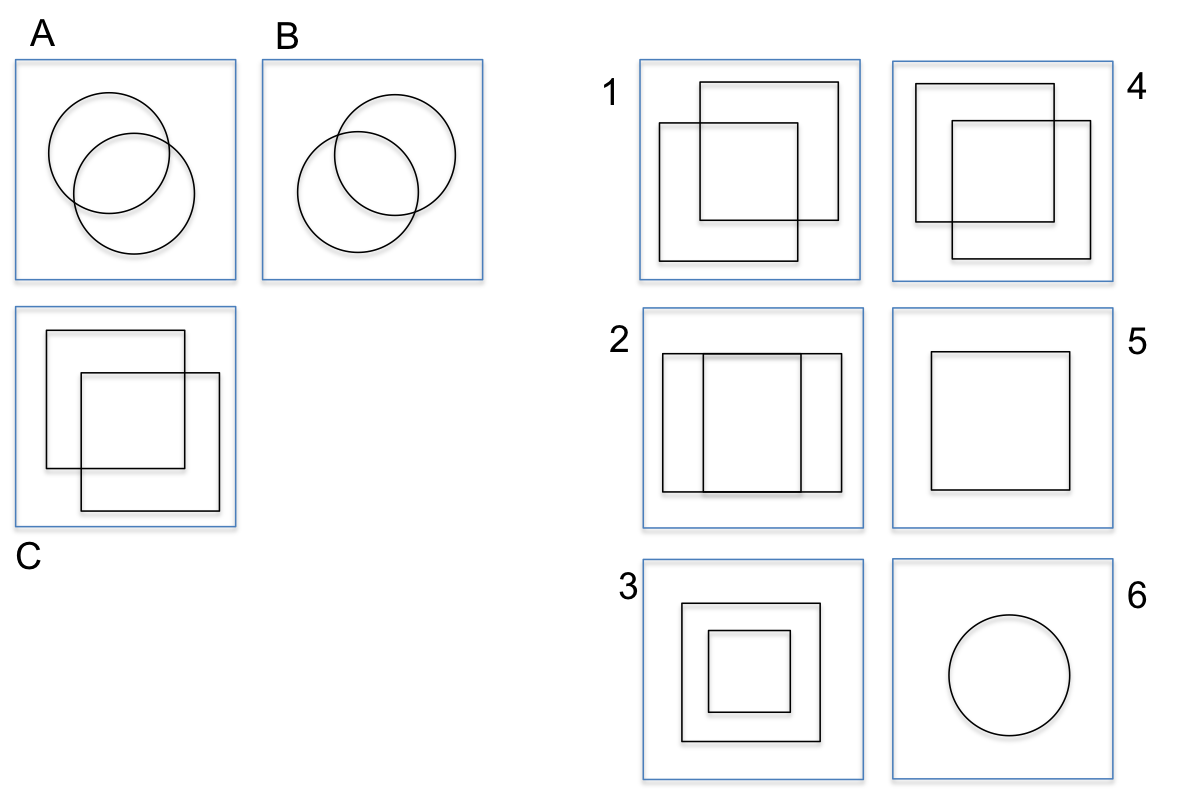
\includegraphics[width=4in]{./figures/fig1.png}
\caption{Visual analogy problem exposing a limitation of the current iteration of our agent\label{fig1}}
\end{figure}

\item The currently version of our agent will also fail to highlight the optimal correct answer where semantic differences of an image pair have a higher semantic value. For example, if semantic difference contains {\small \tt\{"angle": "0", "angle": "180"\}}, it can combine to mean "reflection" (depending on the shape). Without explicit coding of these heuristics, however, our AI agent will not come up with this higher semantic meaning on its own.
\end{enumerate}

\rubric{What improvements could you make to your agent given unlimited time and resources? How would you implement those improvements? Would those improvements improve your agent's accuracy, efficiency, generality, or something else?}
Two potential improvements, derived from the above descriptions of the limitations could be made with additional time and resources.
\begin{enumerate}
\item As long as the agent depends on verbal descriptions, its accuracy can be improved by hardcoding some common heuristics into its logic. An example would be to recognize that for some shapes a 180 degree rotation is equivalent to reflection. This would allow the agent to emphasize answers with lower cognitive weight. 

\item In the long run (definitely by Project 3 !) we'd like to lift our agent's dependency on verbal descriptions. This will allow us to address a much wider range of problems.
\end{enumerate}
%%
\rubric{How well does your agent perform across multiple metrics? Accuracy is important, but what about efficiency? What about generality? Are there other metrics or scenarios under which you think your agent?s performance would improve or suffer?}
Our agent is able to achieve a set-level accuracy of 5.75 in a running time of 0.1 seconds. As detailed above, the agent's performance would suffer if answer choices differ in aspects not captured by the verbal descriptions. Generally, we'd expect an agent relying purely on verbal descriptions to be extremely fast.
%%
\rubric{Which reasoning method did you choose? Are you relying on verbal representations or visual? If you?re using visual input, is your agent processing it into verbal representations for subsequent reasoning, or is it reasoning over the images themselves?}
The present iteration of our agent is using verbal descriptions. Its reasoning process and algorithm is described in detail in the answer to the first question. 
%%
\rubric{Finally, what does the design and performance of your agent tell us about human cognition? Does your agent solve these problems like a human does? How is it similar, and how is it different? Has your agent?s performance given you any insights into the way people solve these problems?}

The process followed by our agent symbolically emulates how I personally approach the Raven's problems. I try to abstract out the core differences between an image-pair and ``add'' that difference to the third image to get the final answer. Our agent works similarly but, of course, needs to represent these cognitive differences explicitly. For example, our agent discards anything common to both images and retains only those things that are unique to each image. Once it has quantified the dissimilarity between an image pair (A and B), something we're termed ``semantic difference'', it looks for answer choices that have a a similar degree of dissimilarity with the third image (C). 

However, the current iteration of our agent is not able to capture aesthetics. For example, it performs poorly on Basic Problem B-4 because the optimal answer ``completes the square''. In a sense, it seems that human cognition is able to account for ``long rage order'' in solving problems, which our agent cannot. 

In addition, I'm finding spatial reasoning comes naturally to me, while it is hard to code into the agent. 
\end{document}












